\chapter{Experimentación y resultados}

Una vez construido, validado e implementando el simulador, es momento de la experimentación y del análisis de resultados. A lo largo de este capitulo se exponen los tres principales experimentos realizados utilizando el simulador para generar evoluciones con un autómata celular neuronal y posteriormente las evoluciones son analizadas en Mathematica. 

\section{Duplicación de reglas}

El objetivo de este primer experimento es poder replicar el comportamiento de evoluciones conocidas para identificar la capacidad del autómata celular neuronal de replicar comportamientos con base en su evolución y su vecindad.

Las pruebas a continuación fueron realizadas en un espacio de $100 \times 100$ con una configuración inicial aleatoria y unicamente dos estados. Adelante se muestra el proceso de cada experimento y los resultados obtenidos.

\subsection{Experimento 1: Juego de la vida}

Este experimento analiza diferentes configuraciones del juego de la vida incluyendo la regla original B3/S23. Para el entrenamiento de la red neuronal se usaron 100 pasos evolutivos con una vecindad de $3 \times 3$.

% En esta parte vamos a definir la perdida objetivo

Primero vamos a definir una perdida objetivo,  y de aquí sale una pregunta, ¿Como medimos que 2 reglas son similiares? por consecuente, saber la diferencia entre dos reglas dadas nos permitiria no solo saber si el autoamta celular neuronal fue capaz de replicar correctamente, sino si tan solo fue capaz de extraer las caracteristicas esenciales de dicha regla. A continuación se muestra un ejemplo que nos permite aproximar 

La figura \ref{fig:life_pattern_count} muestra la probabilidad de que aparezca cada patrón en una evolución del juego del juego de la vida con una condición inicial aleatoria. 

\begin{figure}[H]
	\centering
	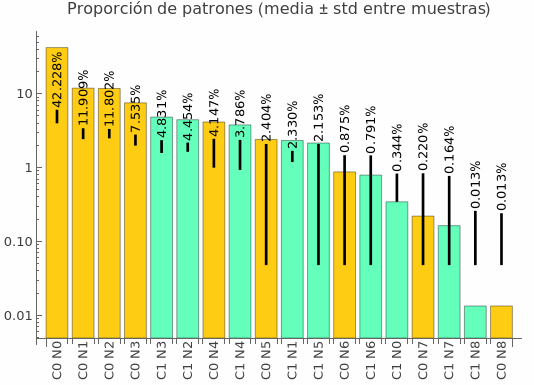
\includegraphics[width=0.7\linewidth]{img/life_pattern_count.png}
	\caption{}
	\label{fig:life_pattern_count}
\end{figure}

\subsubsection{B3/S23}

Considerando una red neuronal de 9 neuronas en la capa de entrada se probaron 10 combinaciones de funciones de activación, de las cuales una sola converge en menos de 1000 épocas, tal como se observa en la tabla \ref{tab:nca_gol_funciones_1}. La falta de convergencia puede deberse al tamaño de la red neuronal o la perdida objetivo utilizada. 

\begin{table}[h]
	\centering
	\begin{tabular}{llrrr}
		\toprule
		\textbf{Capa Oculta} & \textbf{Capa Salida} & \textbf{Épocas} & \textbf{Pérdida} & \textbf{Tiempo} \\
		\midrule
		1:4:ReLU & 2:Linear & 122 & 0.000098 & 4.64 s \\
		1:4:TanH & 1:Sigmoid & 1000 & 0.052895 & 40.19 s\\
		1:4:TanH & 2:Linear & 1000 & 0.079425 & 36.52 s \\
		1:4:Sigmoid & 2:Linear & 1000 & 0.159343 & 36.71 s \\
		1:4:Sigmoid & 1:Sigmoid & 1000 & 0.159343 & 39.37 s \\
		1:4:ReLU & 2:TanH & 1000 &  0.179589 & 38.65 s \\
		1:4:ReLU & 1:Sigmoid & 1000 & 0.269196 & 38.16 s\\
		1:4:Linear & 1:Sigmoid & 1000 & 0.297529 & 39.12 s \\
		1:4:Linear & 2:Linear & 1000 & 0.297529 & 34.75 s  \\
		1:4:ReLU & 2:Sigmoid & 1000 & 0.374756 & 37.55 s \\
		\midrule
	\end{tabular}
	\caption{Comparativa de rendimiento con múltiples hiperparámetros: Perdida objetivo 0.0001, limite de épocas: 1000, 
		tamaño del lote: 8192, tasa de aprendizaje: 0.001, semilla aleatoria: 42}
	\label{tab:nca_gol_funciones_1}
\end{table}

Si incrementamos el numero de capas ocultas y de neuronas, se observa que en la tabla \ref{tab:nca_gol_funciones_2} ahora existen cinco configuraciones que alcanzan la convergencia. Adicionalmente, en la figura \ref{fig:gol_funciones_2} observamos que el estancamiento ocurre en las primeras 12 épocas, lo que sugiere que se deba a la tasa de aprendizaje. 

\begin{table}[h]
	\centering
	\begin{tabular}{llrr}
		\toprule
		\textbf{Capa Oculta} & \textbf{Capa Salida} & \textbf{Épocas} & \textbf{Pérdida}\\
		\midrule
		4:8:ReLU & 2:Linear & 18 & 0.000087 \\
		4:8:TanH & 1:Sigmoid & 51 & 0.000097 \\
		4:8:TanH & 2:Linear & 35 & 0.000097 \\
		4:8:Sigmoid & 2:Linear & 79 & 0.000095 \\
		4:8:Sigmoid & 1:Sigmoid & 1000 & 0.159342 \\
		4:8:ReLU & 2:TanH & 1000 & 0.126928 \\
		4:8:ReLU & 1:Sigmoid & 133 & 0.000096 \\
		4:8:Linear & 1:Sigmoid & 1000 & 0.297542 \\
		4:8:Linear & 2:Linear & 1000 & 0.297544 \\
		4:8:ReLU & 2:Sigmoid & 1000 & 0.374756 \\
		\bottomrule
	\end{tabular}
	\caption{Comparativa de rendimiento con múltiples hiperparámetros: Perdida objetivo 0.0001, limite de épocas: 1000, 
		tamaño del lote: 8192, tasa de aprendizaje: 0.001, semilla aleatoria: 42}
	\label{tab:nca_gol_funciones_2}
\end{table}

\begin{figure}[H]
	\centering
	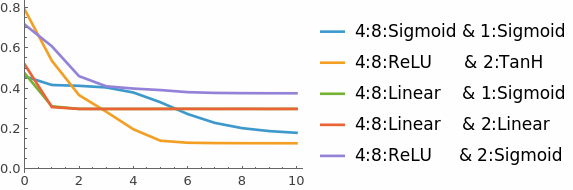
\includegraphics[width=0.75\linewidth]{img/gol_funciones_2.png}
	\caption{Registro de perdida obtenida en los primeros 12 pasos de las configuraciones sin convergencia}
	\label{fig:gol_funciones_2}
\end{figure}

Al haber encontrado configuraciones de la red neuronal que son capaces de converger con un perdida de 0.0001, no resulta necesario experimentar con el resto de configuraciones, pues los próximos experimentos serán desarrollados con las redes neuronales descubiertas. 

\subsubsection{NCA multicapa: B3/S236}


las figuras \ref{fig:ex_1} muestran la comparativa de estas reglas con respecto a la evolución base. Claramente se observa que todas las reglas generadas por esas condiciones tienden a generar combinaciones estáticas. Por lo que no tienen parecido a la regla B3/S23.

\begin{figure}[!htbp]
	\centering
	\begin{subfigure}[b]{0.7\linewidth}
		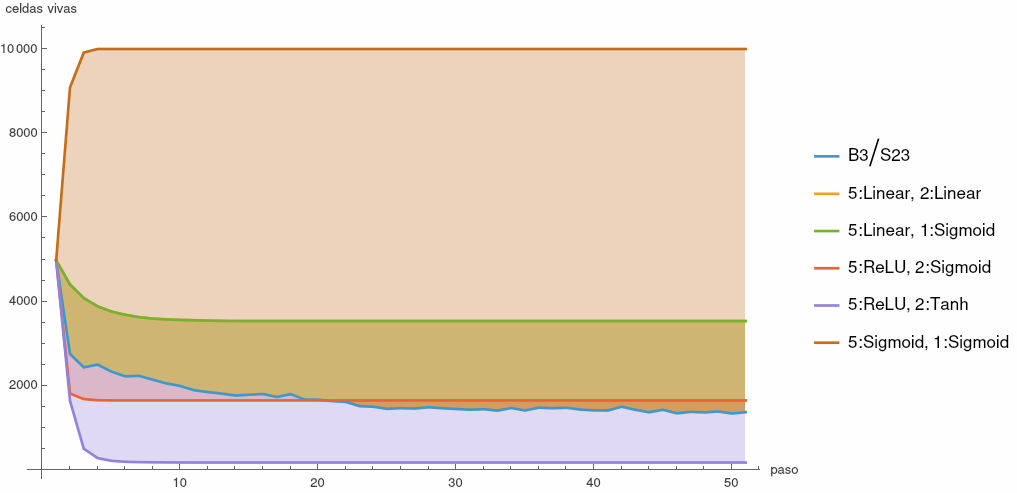
\includegraphics[width=\textwidth]{img/ex_1_ones.png}
		\caption{Regla B2/S23}
		\label{fig:ex_1_ones}
	\end{subfigure}
	\begin{subfigure}[b]{0.7\linewidth}
		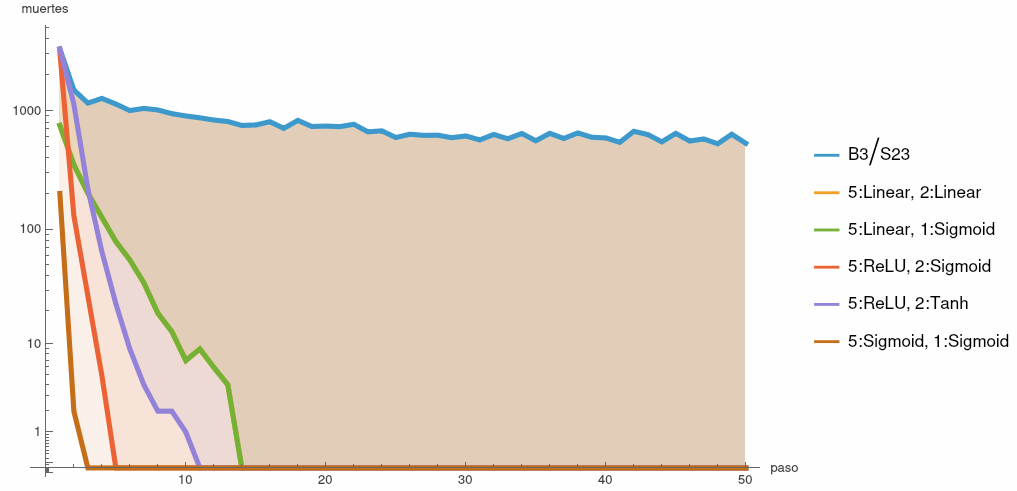
\includegraphics[width=\textwidth]{img/ex_1_death.png}
		\caption{Regla B2/S23}
		\label{fig:ex_1_death}
	\end{subfigure}
	\begin{subfigure}[b]{0.7\linewidth}
		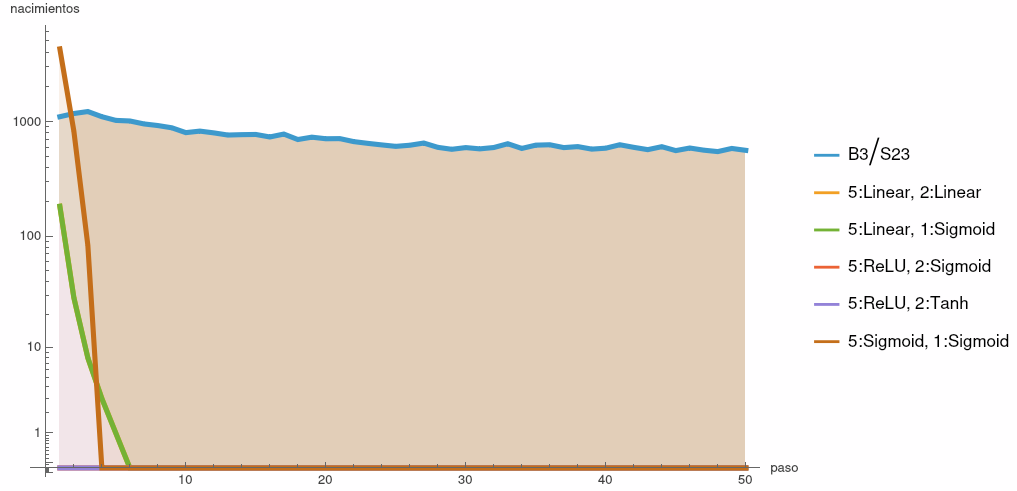
\includegraphics[width=\textwidth]{img/ex_1_born.png}
		\caption{Regla B2/S23}
		\label{fig:ex_1_born}
	\end{subfigure}
	\begin{subfigure}[b]{0.7\linewidth}
		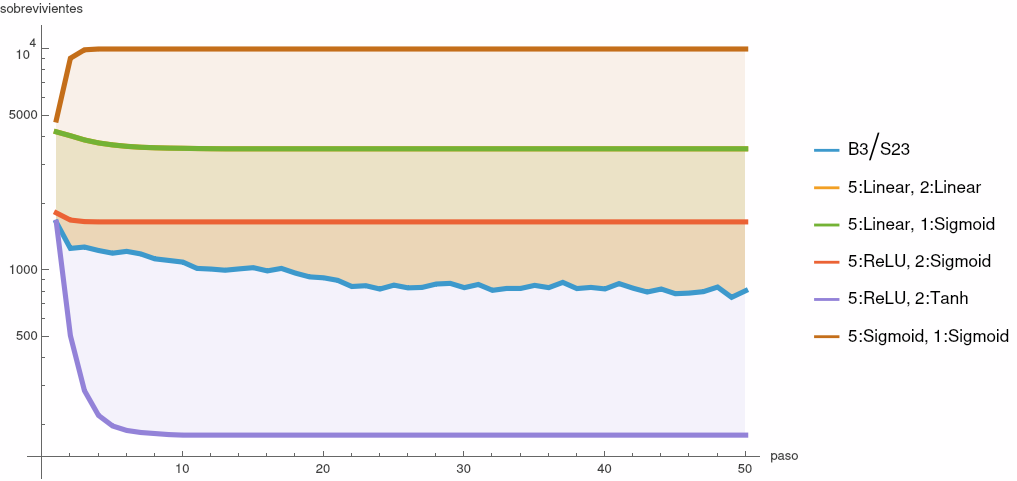
\includegraphics[width=\textwidth]{img/ex_1_live.png}
		\caption{Regla B2/S23}
		\label{fig:ex_1_live}
	\end{subfigure}
	\caption{sas}
	\label{fig:ex_1}
\end{figure}

Para poner a prueba el potencial de las redes neuronales, se realiza la prueba de las mismas funciones de activación pero incrementando el numero de capas y aplicándolo a la regla B3/S236. Los resultados obtenidos se encuentran en la tabla \ref{tab:nca_gol_funciones_2}, de las cuales solo las ultimas dos funciones no fueron capaces de replicar el comportamiento.

\begin{table}[h]
	\centering
	\begin{tabular}{llrr}
		\toprule
		\textbf{Capa Oculta} & \textbf{Capa Salida} & \textbf{Épocas} & \textbf{Pérdida} \\
		\midrule
		(4) 64:ReLU & 2:TanH & 2000 & 0.146712 \\
		(4) 64:ReLU & 2:Sigmoid & 2000 & 0.323128 \\
		(4) 64:Sigmoid & 1:Sigmoid & 2000 & 0.323180 \\
		(4) 64:Linear & 1:Sigmoid & 2000 & 0.483726 \\
		(4) 64:Linear & 2:Linear & 2000 & 0.515534 \\
		\bottomrule
	\end{tabular}
	\caption{Comparativa de hiperparámetros y desempeño del modelo. La pérdida representa el valor final tras alcanzar la convergencia o el límite de épocas.}
	\label{tab:nca_gol_funciones_3}
\end{table}

Podemos corroborar esta información con las graficas de las figuras \ref{fig:ex_2}. Esto nos deja una nueva pregunta: Cual es el limite de la perdida aceptable para que un autómata celular neuronal pueda replicar el comportamiento de su contraparte original?

\begin{figure}[!htbp]
	\centering
	\begin{subfigure}[b]{0.7\linewidth}
		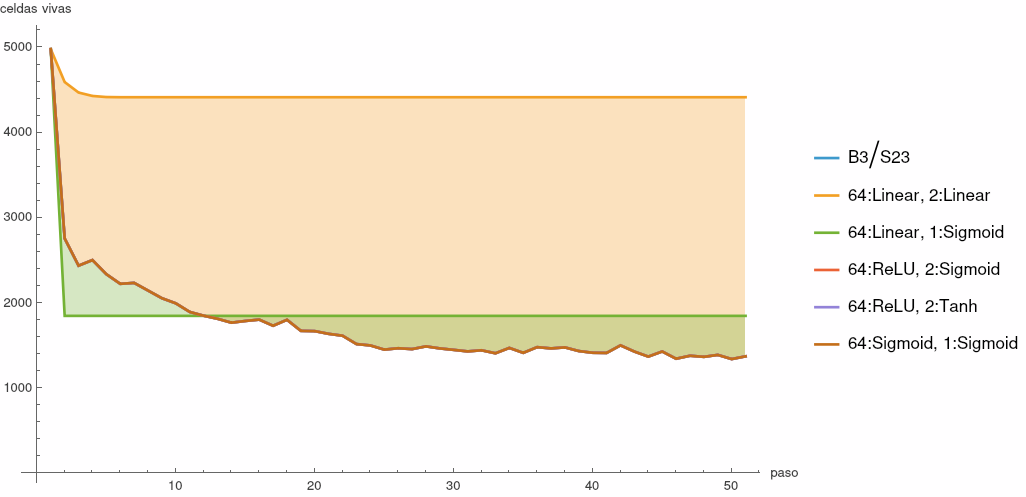
\includegraphics[width=\textwidth]{img/ex_2_ones.png}
		\caption{Regla B2/S23}
		\label{fig:ex_2_ones}
	\end{subfigure}
	\begin{subfigure}[b]{0.7\linewidth}
		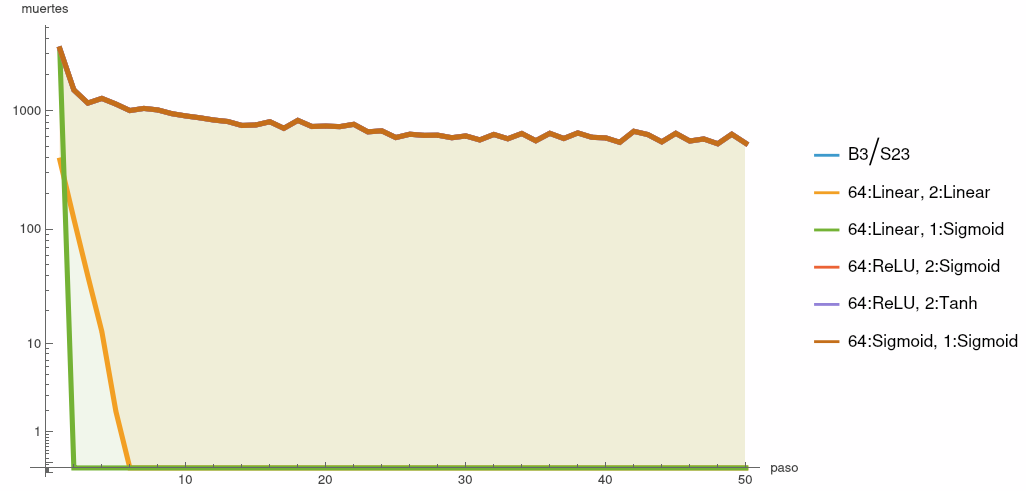
\includegraphics[width=\textwidth]{img/ex_2_death.png}
		\caption{Regla B2/S23}
		\label{fig:ex_2_death}
	\end{subfigure}
	\begin{subfigure}[b]{0.7\linewidth}
		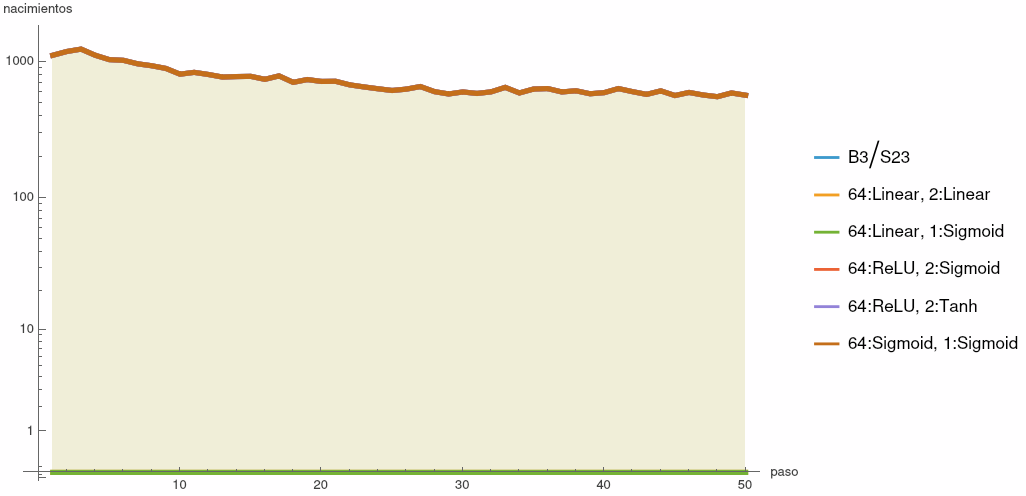
\includegraphics[width=\textwidth]{img/ex_2_born.png}
		\caption{Regla B2/S23}
		\label{fig:ex_2_born}
	\end{subfigure}
	\begin{subfigure}[b]{0.7\linewidth}
		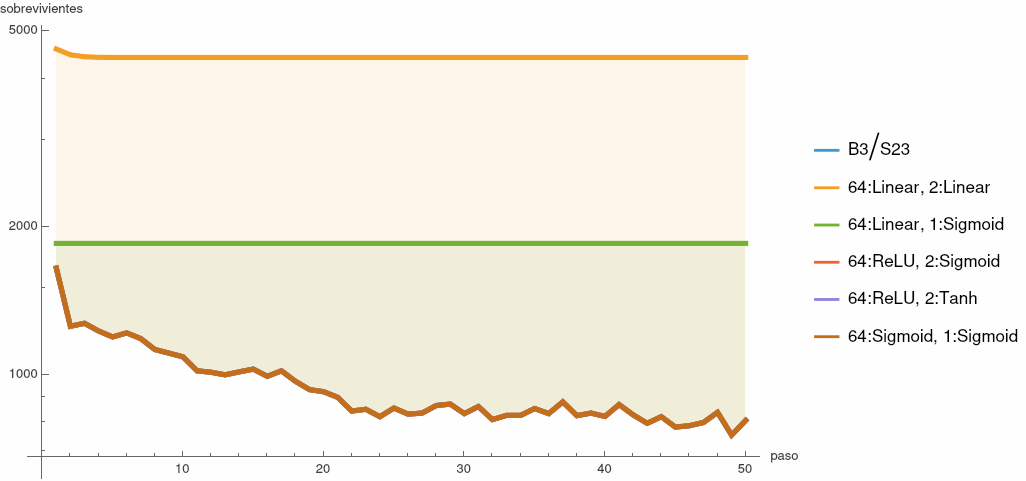
\includegraphics[width=\textwidth]{img/ex_2_live.png}
		\caption{Regla B2/S23}
		\label{fig:ex_2_live}
	\end{subfigure}
	\caption{sas}
	\label{fig:ex_2}
\end{figure}


Finalmente, podemos tener una convergencia casi inmediata si utilizamos la configuración 32:ReLU, 32:ReLU, 2:Linar, teniendo una perdida de 0.001048.


\subsubsection{Variación de error}

Para intentar responder esta nueva pregunta, se realizo un nuevo entrenamiento con la configuración 5:Sigmoid, 2:Linear por ser capaz de converger y de reducir gradualmente la perdida, esto se hace para poder aproximarse aún mas a la perdida objetivo y no rebasarla por completo.

Se realizaron 19 pruebas variando la tasa de error aceptable entre 0.001 y 0.1. En la figura \ref{fig:perdida_objetivo} se muestra como los NCA con una tasa de error de 0.001 y 0.002 replicaron el comportamiento de B3/S236, sin embargo, cualquier tasa de aprendizaje superior difiere de la regla original. Adicionalmente se encontró que si definimos una tasa de error mayor a 0.03 el comportamiento  que aprende equivale a B3/S23. 

\begin{figure}[H]
	\centering
	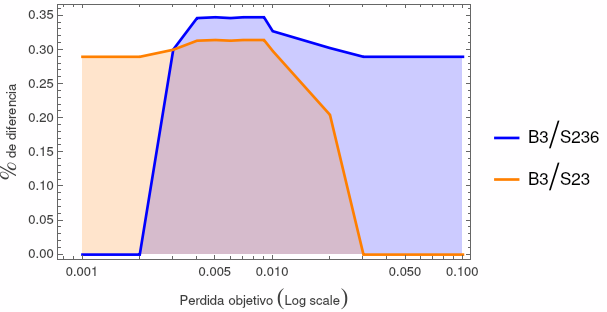
\includegraphics[width=0.95\linewidth]{img/perdida_objetivo.png}
	\caption{Comparativa de Diferencias por Configuración.}
	\label{fig:perdida_objetivo}
\end{figure}

Estas 2 reglas difieren unicamente en un elemento como se muestra en las figuras \ref{fig:rules_life}. Que es cuando la célula central vale 1 (C1) y la vecindad suma 6 (N6). 

\begin{figure}[!htbp]
	\centering
	\begin{subfigure}[b]{0.45\textwidth}
		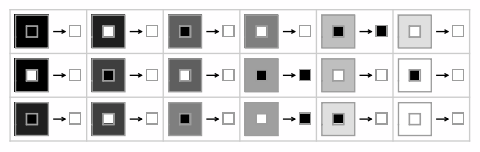
\includegraphics[width=\textwidth]{img/rule_b3_s23.png}
		\caption{Regla B2/S23}
		\label{fig:rule_b3_s23}
	\end{subfigure}
	\begin{subfigure}[b]{0.45\textwidth}
		\includegraphics[width=\textwidth]{img/rule_b3_S236.png}
		\caption{Regla B2/S23}
		\label{fig:rule_b3_S236}
	\end{subfigure}
	\caption{sas}
	\label{fig:rules_life}
\end{figure}

Si contamos el numero de patrones de interés que se encuentran por evolución, obtenemos que el patrón C1, N6 solo equivale al 0.756133\%, como se muestra en la figura \ref{fig:B2_S236_proportion}, numero menor a la tasa de error aceptable. Por lo que este patrón se considera un error aceptable en la regla B3/S23.

\begin{figure}[H]
	\centering
	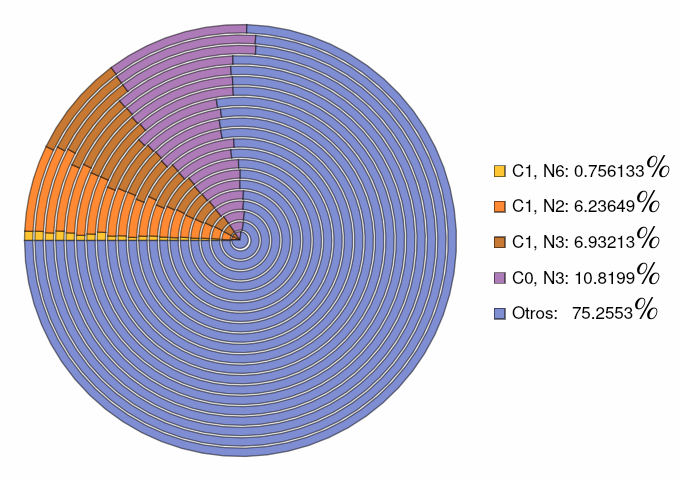
\includegraphics[width=0.95\linewidth]{img/B2_S236_proportion.png}
	\caption{Proporción.}
	\label{fig:B2_S236_proportion}
\end{figure}

Entonces es de esperarse que reduciendo la tasa de error aceptable encontremos configuraciones que contienen mayor similitud. Para lograr esto primero buscamos cuales son las reglas que existen en el intervalo de $[0.003, 0.03]$. 

Para lograr esto, primero se prueban todos los escenarios posibles en la regla y despues se evoluciona el sistema con la misma condición inicial, si la neuva evolución corresponde con la evolución previamente generada por el NCA entonces podemos afirmar que el NCA si aprendio una existente en ese espacio. Por ejemplo, en la figura \ref{fig:b38_s236} se aprecia 100-esima evolución mediante la regla B38/S236 y la regla generada con el NCA usando un 0.003 como error aceptable, por lo que corroboramos que son equivalentes.

\begin{figure}[!htbp]
	\centering
	\begin{subfigure}[b]{0.45\textwidth}
		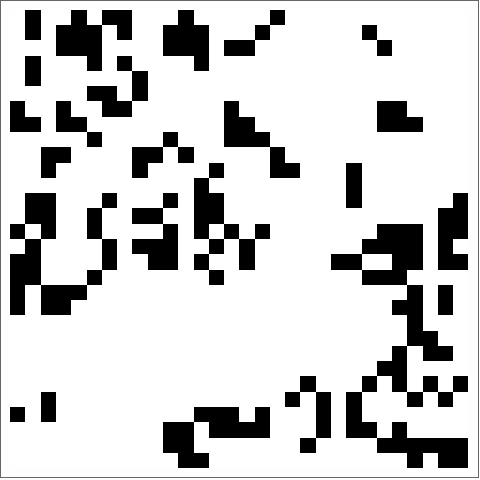
\includegraphics[width=\textwidth]{img/r73952.png}
		\caption{Regla B38/S236}
		\label{fig:r73952}
	\end{subfigure}
	\begin{subfigure}[b]{0.45\textwidth}
		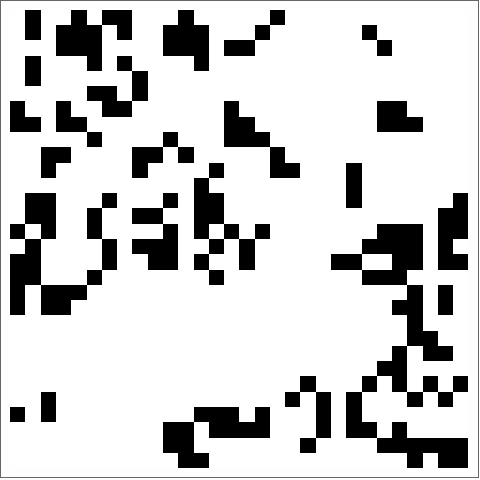
\includegraphics[width=\textwidth]{img/nca003.png}
		\caption{NCA con 0.003}
		\label{fig:nca003}
	\end{subfigure}
	\caption{sas}
	\label{fig:b38_s236}
\end{figure}

Aplicando este mismo proceso, se obtuvieron los resultados de la tabla \ref{tab:nca_asociacion}. En ella se muestra la asociación entre NCA y las reglas de los autómatas celulares. 

\begin{table}[h]
	\centering
	\begin{tabular}{c | c}
		\textbf{Error} & \textbf{Regla} \\ \hline
		0.003 & B38/S236 \\
		0.004 & B3/S23678 \\
		0.005 & B38/S23678  \\
		0.1 & B3/S2368 \\
		0.2 & B3/S2378 \\
	\end{tabular}
	\caption{Proporcion en las reglas obtenidas.}
	\label{tab:nca_asociacion}
\end{table}

Que una regla aprendida haya inferido otra regla puede ser un problema debido a las propiedades caóticas de los autómatas celulares, lo que podría suponer ser lo suficientemente complejos para no poder extraer las reglas con alta precisión.

Sin embargo, esto no siempre es verdadero. Para probar que el NCA tiene una aproximación realizamos las mismas mediciones de conteo de unos, nacimientos, muertes y sobrevivientes sobre multiples evoluciones de la misma regla. Este proceso se realiza multiples veces para evitar el ruido, y finalmente se comparan las graficas. 

En las figuras \ref{fig:error_plot} se muestran las graficas del comportamiento de las 5 reglas mas B3/S23 y B3/S236. 

Observamos entonces que el intercambio que ocurren entre ambas reglas no son comportamientos arbitrario sino que navega entre diferentes reglas. 

\begin{figure}[!htbp]
	\centering
	\begin{subfigure}[b]{0.7\linewidth}
		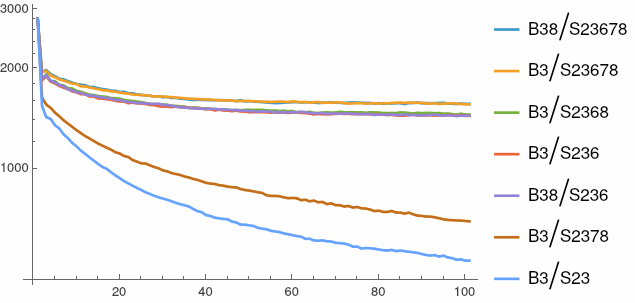
\includegraphics[width=\textwidth]{img/error_plotO.png}
		\caption{Regla B2/S23}
		\label{fig:error_plotO}
	\end{subfigure}
	\begin{subfigure}[b]{0.7\linewidth}
		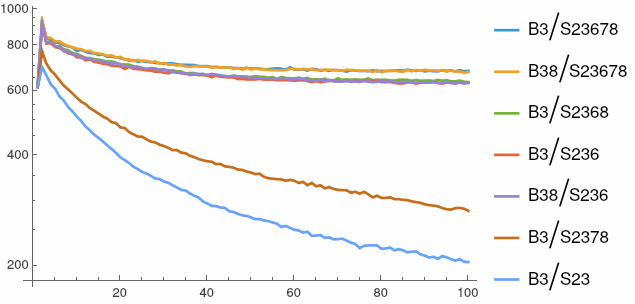
\includegraphics[width=\textwidth]{img/error_plotB.png}
		\caption{Regla B2/S23}
		\label{fig:error_plotB}
	\end{subfigure}
	\begin{subfigure}[b]{0.7\linewidth}
		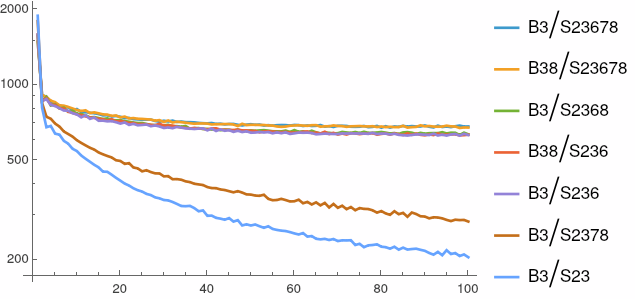
\includegraphics[width=\textwidth]{img/error_plotD.png}
		\caption{Regla B2/S23}
		\label{fig:error_plotD}
	\end{subfigure}
	\begin{subfigure}[b]{0.7\linewidth}
		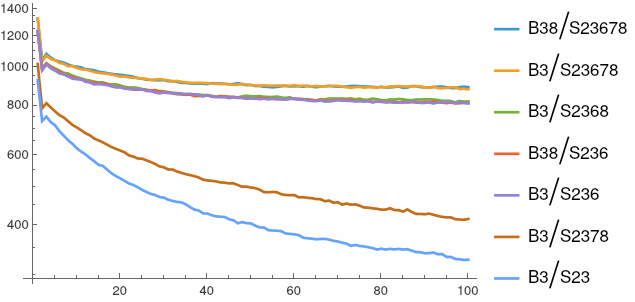
\includegraphics[width=\textwidth]{img/error_plotL.png}
		\caption{Regla B2/S23}
		\label{fig:error_plotL}
	\end{subfigure}
	\caption{sas 2}
	\label{fig:error_plot}
\end{figure}

Podemos concluir que la tasa de error aceptable es un parámetro que tiene mucha influencia en la evolución, pero que pese a que cambien sus valores su comportamiento aunque no lo logre replicar exactamente el mismo comportamiento, si es capaz de obtener un comportamiento lo suficientemente similar como para llegar a casi indistinguibles. 

Es necesario recordar que estos resultados corresponden unicamente al experimento que existen entre dos reglas, la regla B3/S23 y B3/S236 y todas las reglas adicionales descubiertas en el camino. Esto ya que el mismo comportamiento de reglas similares o con mismos comportamientos que obliguen a disminuir la tasa de error puede que no existan o que incluso se aplique a todos ellas, esta parte del experimento busca unicamente demostrar que aunque las variaciones de la tasa de error aceptable puedan generar comportamientos diferentes (como normalmente pasaría en cualquier red neuronal), no tiene implicaciones a gran escala ya que la regla aprendida sigue siendo similar a la regla con la que fue entrenada, ademas, solo se están considerando cuatro parámetros para determinar la similitud entre dos reglas.

Replicar reglas conocidas es muy sencillo porque sabemos exactamente cual va a ser el comportamiento. Y aunque existen reglas que tienen comportamientos similares, al final tenemos todas la información suficiente. Pero ¿Qué pasa cuando carecemos de toda la información? En los siguientes experimentos intentamos responder a esas preguntas limitando el conocimiento del autómata celular neuronal.

\subsection{Experimento 2: Vecindad desconocida}

Como se ha observado hasta el momento, los unicos datos requeridos para poder definir al automata celular neuronal es la evolución y la vecindad. Con esto nos surge una pregunta, ¿Que ocurre cuando no conocemos la vecindad? La opción obvio es incrementar la vecindad lo suficiente para que pueda encontrar estos patrones, pero en este experimento el objetivo es forzar el desconocimiento de un elemento e identificar si el incremento de la vecindad puede compensar esa falta. 

La primera parte de este experimento es en reglas con vecindades pequeñas, como son los ECA de Wolfram. Antes hay que extrapolar el comportamiento del ECA en dos dimensiones, para eso se usa el kernel de la figura \ref{fig:eca_neighbourhood}. En donde la vecindad se coloca un escalón arriba, haciendo que la evolución se propague hacia abajo (notese que no existe la persistencia de los datos).

\begin{figure}[H]
	\centering
	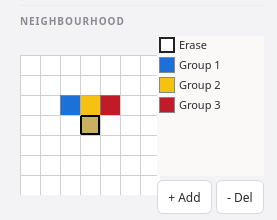
\includegraphics[width=0.95\linewidth]{img/eca_neighbourhood.png}
	\caption{Proporción.}
	\label{fig:eca_neighbourhood}
\end{figure}

Con esto, ya podemos simular cualquier ECA. Para corroborar el funcionamiento del NCA primero se generó una regla capaz de replicar la regla 90. Utilizando un kernel de $3 \times 3$ 3:ReLu, 2:Linear convergió en 68 epocas y una perdida de 0.000966.

Limitando la vecindad a lo que realmente es bajo la misma configuración tenemos que converge en 53 epocas y una perdida de 0.000965.

Si utilizamos toda la linea horizontal, tenemos una convergencia en 65 epocas con una perdida de 0.000945.

Y con esta regla podemos omitir la célula central, ya que al ver su representación en la figura \ref{fig:ex2_eca90}, da igual el valor que exista en medio.

\begin{figure}[H]
	\centering
	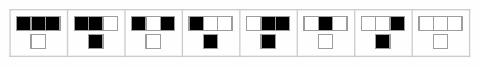
\includegraphics[width=0.95\linewidth]{img/ex2_eca90.png}
	\caption{Proporción.}
	\label{fig:ex2_eca90}
\end{figure}

